% QCML Geometric Observatory — Pipeline Architecture Diagram
% Compile: pdflatex pipeline_diagram.tex
\documentclass[border=12pt]{standalone}
\usepackage[T1]{fontenc}
\usepackage{lmodern}
\usepackage{amsmath,amssymb}
\usepackage{tikz}
\usetikzlibrary{arrows.meta, positioning, shadows.blur, calc, fit}

% ── Color palette (matches plot_style.py) ──
\definecolor{navy}{HTML}{1B2A4A}
\definecolor{teal}{HTML}{2D6A6A}
\definecolor{burgundy}{HTML}{8B2252}
\definecolor{gold}{HTML}{C9A84C}
\definecolor{indigo}{HTML}{4B3F72}
\definecolor{slate}{HTML}{64748B}
\definecolor{light}{HTML}{F8F6F0}

% ── Styles ──
\tikzset{
  % Main pipeline boxes
  stage/.style={
    draw=navy, fill=light, rounded corners=4pt,
    minimum width=11cm, minimum height=1.3cm,
    font=\sffamily, text=navy, align=center,
    blur shadow={shadow blur steps=5, shadow xshift=0.8pt,
                 shadow yshift=-0.8pt, shadow opacity=15},
  },
  stage title/.style={font=\sffamily\bfseries\small, text=navy},
  stage body/.style={font=\small, text=slate},
  % Observable boxes
  obs/.style={
    draw=#1, fill=#1!8, rounded corners=3pt,
    minimum width=2.2cm, minimum height=1.2cm,
    font=\sffamily\small, text=navy, align=center,
    blur shadow={shadow blur steps=4, shadow xshift=0.6pt,
                 shadow yshift=-0.6pt, shadow opacity=12},
  },
  obs/.default=navy,
  % Arrows
  pipe/.style={-{Stealth[length=5pt]}, line width=0.8pt, navy},
  fan/.style={-{Stealth[length=4pt]}, line width=0.6pt, slate},
  % Labels on arrows
  arrlabel/.style={font=\sffamily\scriptsize, text=slate, fill=white,
                   inner sep=1.5pt},
}

\begin{document}
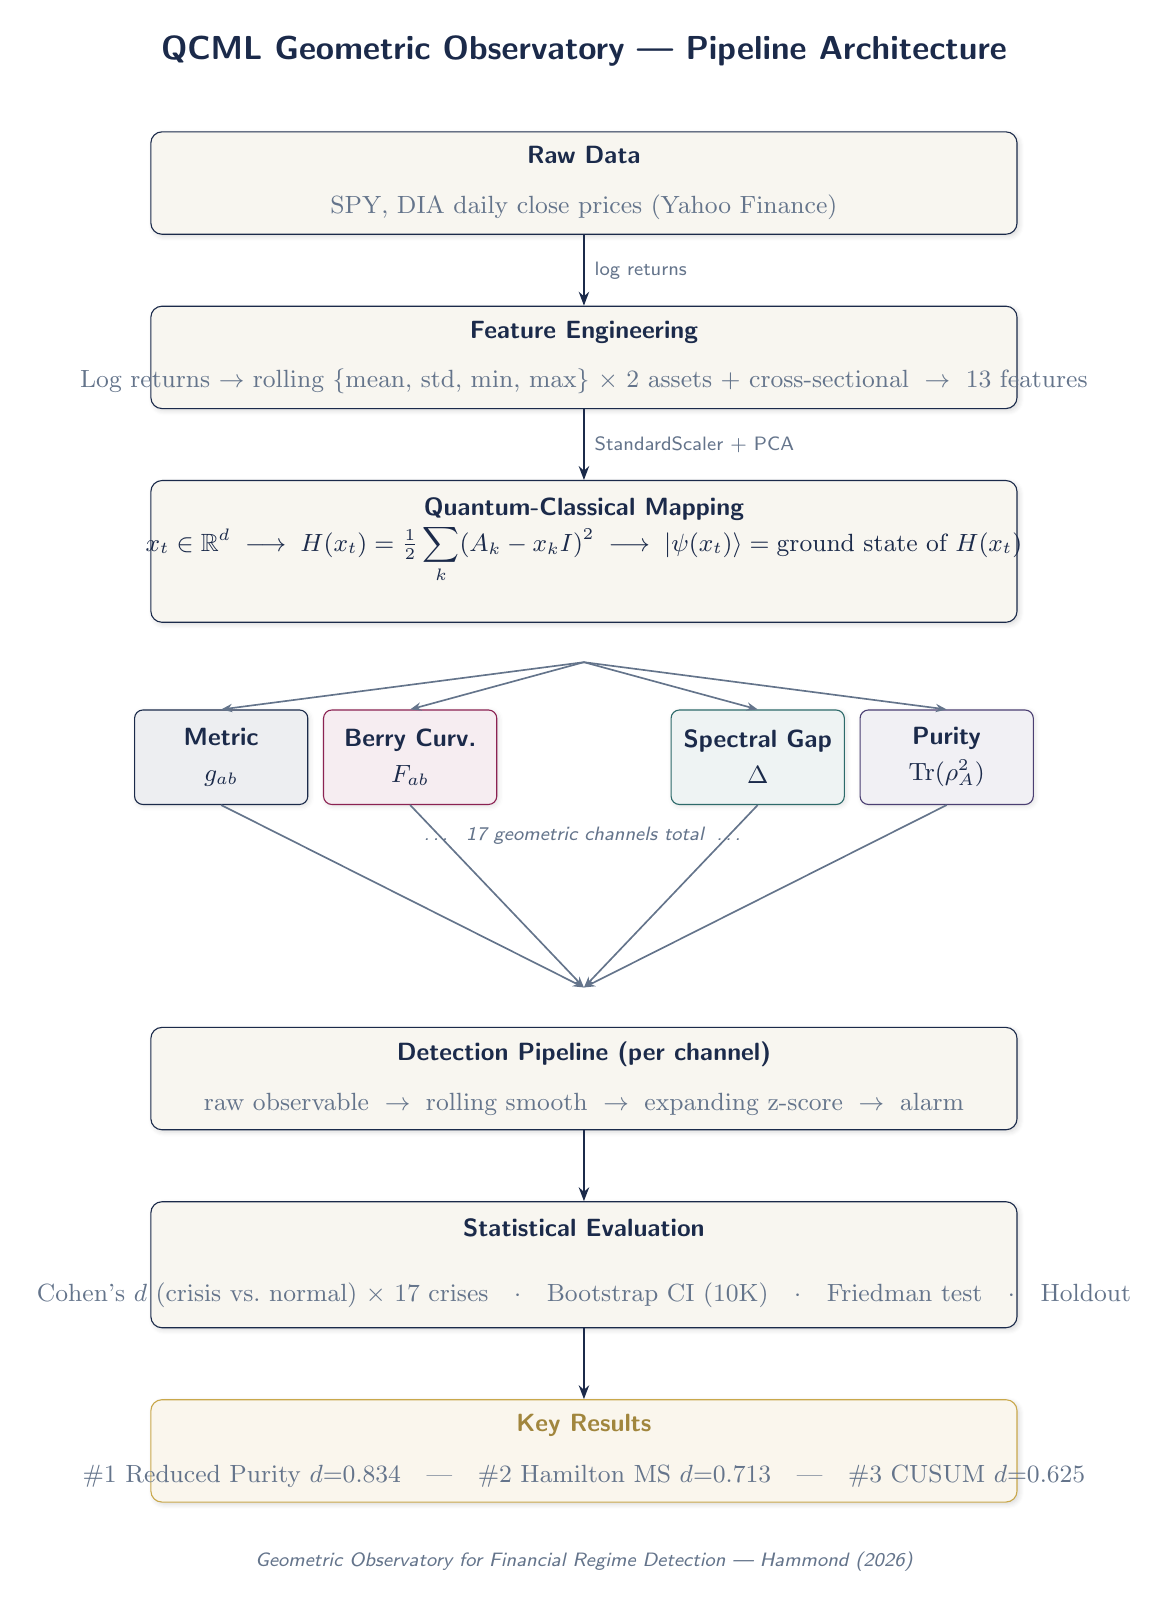
\begin{tikzpicture}[node distance=1.0cm]

% ====================================================================
% Title
% ====================================================================
\node[font=\sffamily\bfseries\large, text=navy] (title)
  {QCML Geometric Observatory --- Pipeline Architecture};

% ====================================================================
% Stage 1: Raw Data
% ====================================================================
\node[stage, below=0.7cm of title] (raw) {};
\node[stage title, anchor=north] at ([yshift=-2pt] raw.north)
  {Raw Data};
\node[stage body, anchor=south] at ([yshift=2pt] raw.south)
  {SPY, DIA daily close prices (Yahoo Finance)};

% ====================================================================
% Stage 2: Feature Engineering
% ====================================================================
\node[stage, below=0.9cm of raw] (feat) {};
\node[stage title, anchor=north] at ([yshift=-2pt] feat.north)
  {Feature Engineering};
\node[stage body, anchor=south] at ([yshift=2pt] feat.south)
  {Log returns $\to$ rolling \{mean, std, min, max\} $\times$ 2 assets $+$ cross-sectional $\;\to\;$ 13 features};

\draw[pipe] (raw) -- node[arrlabel, right=2pt] {log returns} (feat);

% ====================================================================
% Stage 3: Quantum-Classical Mapping
% ====================================================================
\node[stage, minimum height=1.8cm, below=0.9cm of feat] (qcmap) {};
\node[stage title, anchor=north] at ([yshift=-3pt] qcmap.north)
  {Quantum-Classical Mapping};
\node[font=\small, text=navy, anchor=center] at ([yshift=-1pt] qcmap.center)
  {$x_t \in \mathbb{R}^d \;\longrightarrow\;
   H(x_t) = \tfrac{1}{2}\displaystyle\sum_k (A_k - x_k I)^2
   \;\longrightarrow\; |\psi(x_t)\rangle = \text{ground state of } H(x_t)$};

\draw[pipe] (feat) -- node[arrlabel, right=2pt] {StandardScaler $+$ PCA} (qcmap);

% ====================================================================
% Stage 4: Observable Fan-out (4 boxes)
% ====================================================================
\coordinate (fanout) at ([yshift=-0.5cm] qcmap.south);

\node[obs=navy, below left=1.1cm and 3.5cm of qcmap.south] (metric) {
  \textbf{Metric}\\[2pt] $g_{ab}$
};
\node[obs=burgundy, below left=1.1cm and 1.1cm of qcmap.south] (berry) {
  \textbf{Berry Curv.}\\[2pt] $F_{ab}$
};
\node[obs=teal, below right=1.1cm and 1.1cm of qcmap.south] (gap) {
  \textbf{Spectral Gap}\\[2pt] $\Delta$
};
\node[obs=indigo, below right=1.1cm and 3.5cm of qcmap.south] (purity) {
  \textbf{Purity}\\[2pt] $\mathrm{Tr}(\rho_A^2)$
};

% Fan-out arrows
\foreach \dest in {metric, berry, gap, purity} {
  \draw[fan] (fanout) -- (\dest.north);
}

% Ellipsis
\node[font=\sffamily\itshape\scriptsize, text=slate,
      below=0.15cm of $(berry.south)!0.5!(gap.south)$]
  (ellipsis) {\ldots\; 17 geometric channels total \;\ldots};

% ====================================================================
% Stage 5: Detection Pipeline
% ====================================================================
\node[stage, below=2.2cm of ellipsis] (detect) {};
\node[stage title, anchor=north] at ([yshift=-2pt] detect.north)
  {Detection Pipeline (per channel)};
\node[stage body, anchor=south] at ([yshift=2pt] detect.south)
  {raw observable $\;\to\;$ rolling smooth $\;\to\;$ expanding z-score $\;\to\;$ alarm};

% Fan-in arrows
\coordinate (fanin) at ([yshift=0.5cm] detect.north);
\foreach \src in {metric, berry, gap, purity} {
  \draw[fan] (\src.south) -- (fanin);
}

% ====================================================================
% Stage 6: Evaluation
% ====================================================================
\node[stage, minimum height=1.6cm, below=0.9cm of detect] (eval) {};
\node[stage title, anchor=north] at ([yshift=-3pt] eval.north)
  {Statistical Evaluation};
\node[stage body, anchor=south] at ([yshift=4pt] eval.south)
  {Cohen's $d$ (crisis vs.\ normal) $\times$ 17 crises\quad$\cdot$\quad
   Bootstrap CI (10K)\quad$\cdot$\quad Friedman test\quad$\cdot$\quad Holdout};

\draw[pipe] (detect) -- (eval);

% ====================================================================
% Stage 7: Key Results
% ====================================================================
\node[stage, fill=gold!10, draw=gold, below=0.9cm of eval] (results) {};
\node[stage title, anchor=north, text=gold!80!black]
  at ([yshift=-2pt] results.north) {Key Results};
\node[stage body, anchor=south] at ([yshift=2pt] results.south)
  {\#1 Reduced Purity $d{=}0.834$\quad|\quad
   \#2 Hamilton MS $d{=}0.713$\quad|\quad
   \#3 CUSUM $d{=}0.625$};

\draw[pipe] (eval) -- (results);

% ====================================================================
% Footer
% ====================================================================
\node[font=\sffamily\itshape\scriptsize, text=slate,
      below=0.5cm of results]
  {Geometric Observatory for Financial Regime Detection --- Hammond (2026)};

\end{tikzpicture}
\end{document}
